\documentclass[10pt,a4paper]{article}
\usepackage[utf8]{inputenc}
\usepackage[magyar]{babel}
\usepackage[T1]{fontenc}
\usepackage{tikz}
\usepackage{pdflscape}
\usepackage[left=2cm,right=2cm,top=2cm,bottom=2cm]{geometry}
\pagenumbering{gobble} 


\begin{document}

\begin{center}
{\Huge \textbf{FELADAT}}
\end{center}

\vspace{0.5cm}

\input{00_LEIRAS.txt}

\newpage
\begin{landscape}
\begin{center}
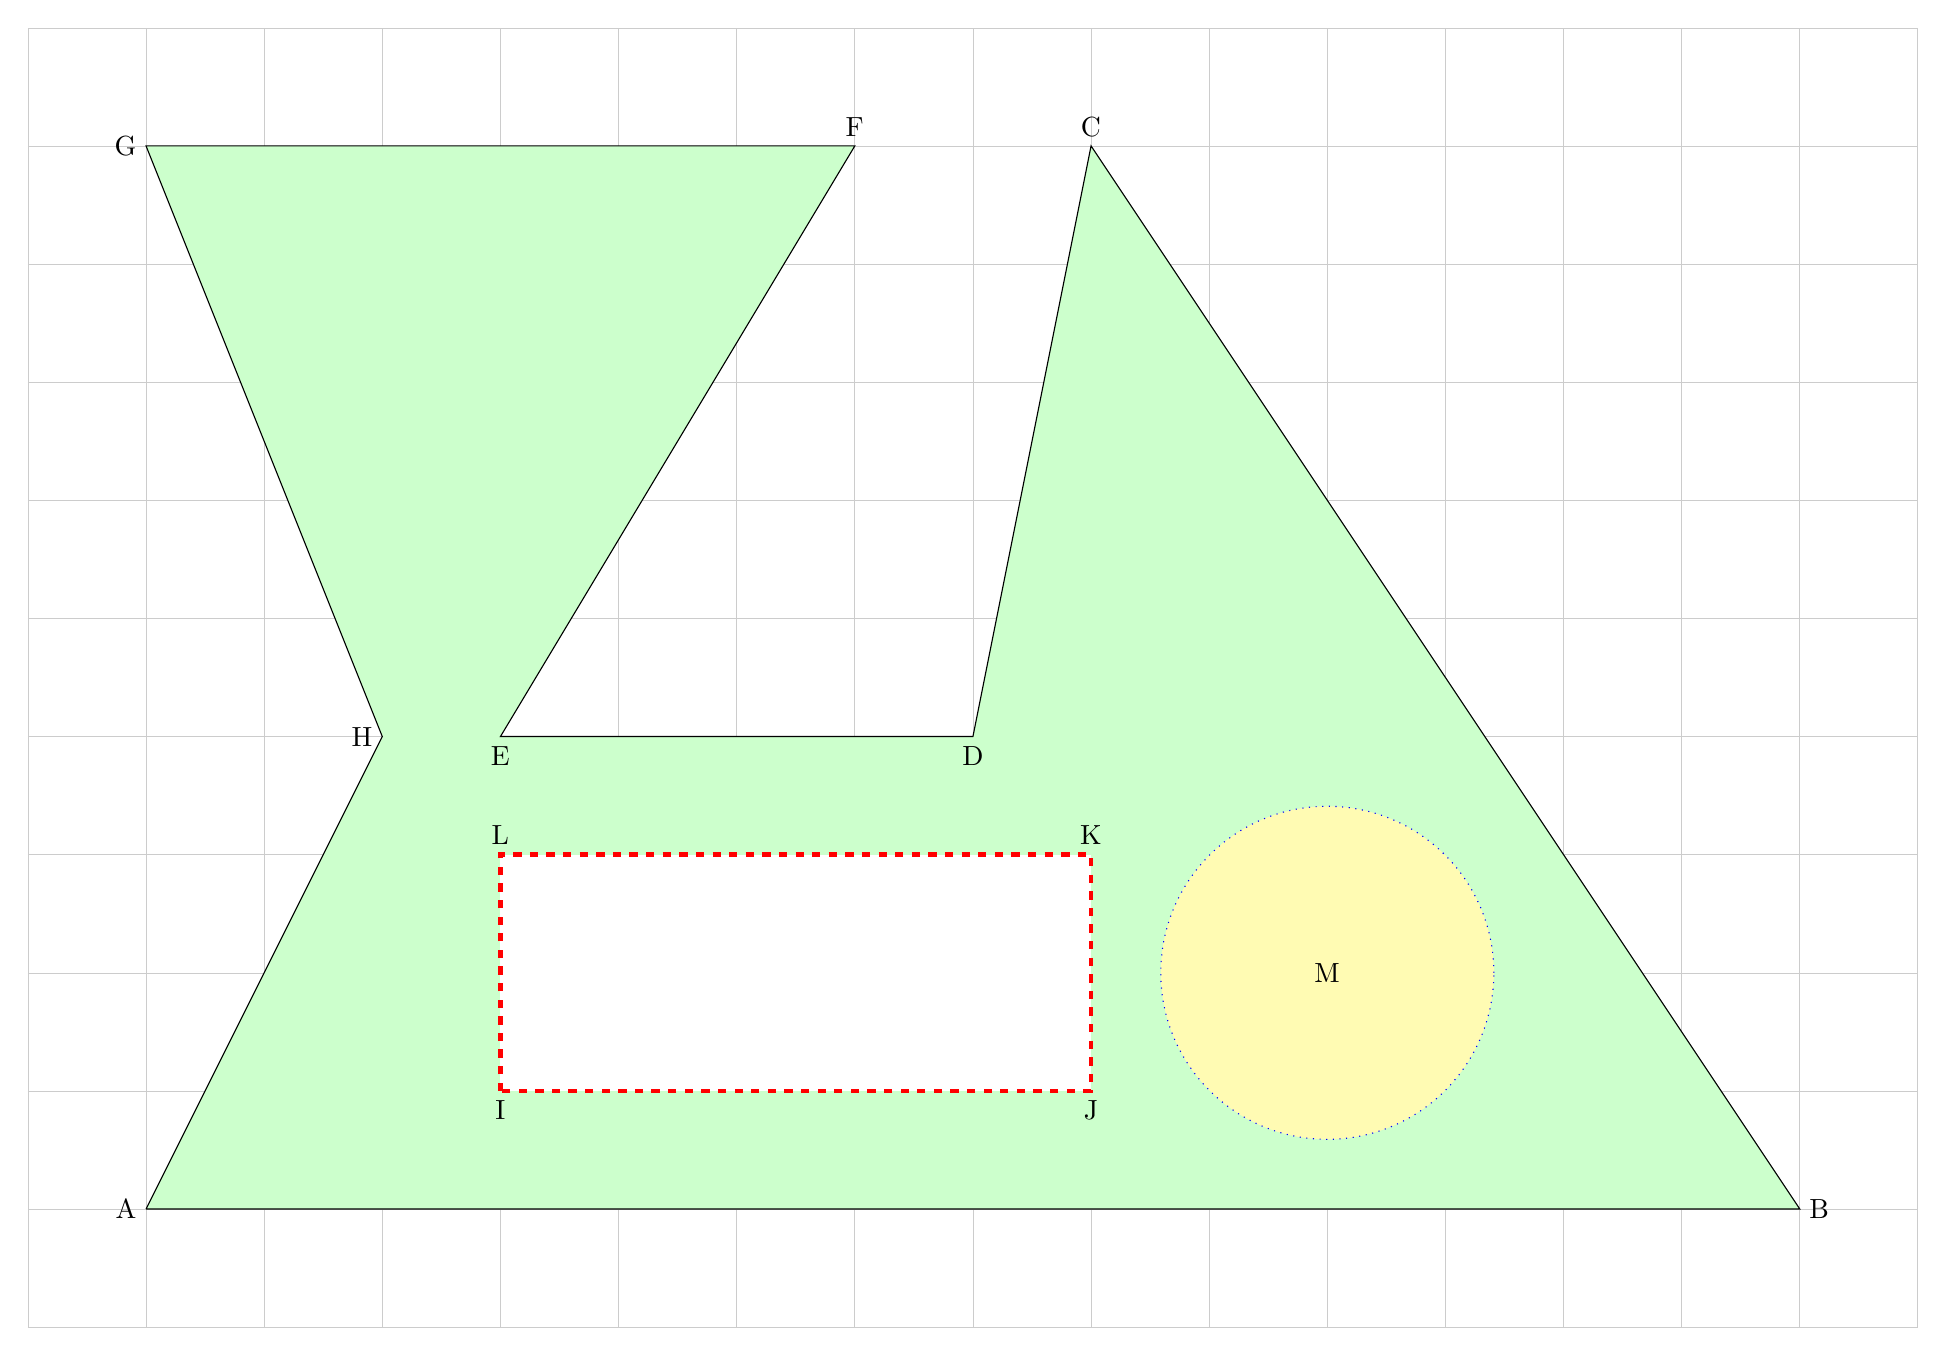
\begin{tikzpicture}[scale=1.5]

\draw [help lines, black!20] (-1,-1) grid (15,10);

\path (0,0) coordinate(A) [left] node {A};
\path (14,0) coordinate(B) [right] node {B};
\path (8,9) coordinate(C) [above] node {C};
\path (7,4) coordinate(D) [below] node {D};
\path (3,4) coordinate(E) [below] node {E};
\path (6,9) coordinate(F) [above] node {F};
\path (0,9) coordinate(G) [left] node {G};
\path (2,4) coordinate(H) [left] node {H};

\path (3,1) coordinate(I) [below] node {I};
\path (8,1) coordinate(J) [below] node {J};
\path (8,3) coordinate(K) [above] node {K};
\path (3,3) coordinate(L) [above] node {L};

\path (10,2) coordinate(M) [] node {M};



\draw [thin, fill=green!20] (A)--(B)--(C)--(D)--(E)--(F)--(G)--(H)--(A);
\draw [ultra thick, dashed, red, fill=white] (I) rectangle (K);
\draw [dotted, blue, fill=yellow!30](M) circle (1.41);

\path (3,1) coordinate(I) [below] node {I};
\path (8,1) coordinate(J) [below] node {J};
\path (8,3) coordinate(K) [above] node {K};
\path (3,3) coordinate(L) [above] node {L};

\path (10,2) coordinate(M) [] node {M};

\path (7,4) coordinate(D) [below] node {D};
\path (3,4) coordinate(E) [below] node {E};

\end{tikzpicture}
\end{center}
\end{landscape}

\newpage
\begin{tikzpicture}[scale=2,xscale=1.2]
\draw [help lines, black!10] (-1,-1) grid (6,11);

\path (0,0) coordinate(A) [below] node {A};
\path (0,10) coordinate(B) [above] node {B};
\path (2,10) coordinate(C) [above] node {C};
\path (0,6) coordinate(D) [left] node {D};
\path (2,6) coordinate(E) [above] node {E};
\path (2,0) coordinate(F) [below] node {F};
\path (1,9) coordinate(G) [left] node {G};
\path (1,7) coordinate(H) [below] node {H};
\path (1,5) coordinate(I) [above] node {I};
\path (1,1) coordinate(J) [left] node {J};
\path (2,5) coordinate(K) [above] node {K};
\path (2,1) coordinate(L) [below] node {L};
\path (2,9) coordinate(M) [above] node {M};
\path (2,7) coordinate(N) [below] node {N};

\draw (F)--(A)--(B)--(C);
\draw (D)--(E);
\draw (L)--(J)--(I)--(K);
\draw (N)--(H)--(G)--(M);

\draw (C) arc (90:-90:2);
\draw (M) arc (90:-90:1);

\draw (K) arc (90:-90:2);
\draw (E) arc (90:-90:3);
\end{tikzpicture}

\end{document}